\documentclass[../../main.tex]{subfiles}

%-----------------------------------------------------------%
\begin{document}
\chapter{Mechanical Sub-system}
\thispagestyle{fancy}

%-----------------------------------------------------------%
% There are two ways to add a section:
%
%
% a) Write the section within the same chapter (Prefer this if the section is small)
%
%
% b) Write a separate section file, and import it to the corresponding chapter (Prefer this if the section is fairly large)
% NOTE: Make sure the names of the (section.tex) are uniquely defined, and easy to read


%\hspace{0.7cm}% 
%----------------------------OR----------------------------%

\subfile{Chapters/Mechanical/mechanical_req}
%----------------------------END----------------------------%

%----------------------------OR----------------------------%

%----------------------------END----------------------------%
\subfile{Chapters/Mechanical/mechanical_config}
\subfile{Chapters/Mechanical/mechanical_mass}
\section{Thermals}
\text Could not be started in near future because of following reasons:
\begin{enumerate}
    \item Requires component level details for thermal inputs in Simulations.
    \item Requires modelling of supporting structures(AUX+PS4OP).
\end{enumerate}
\subfile{Chapters/Mechanical/mechanical_integration}
\newpage
\subfile{Chapters/Mechanical/mechanical_manufacturing}

\section{Peripherals + Auxiliary} 
\begin{enumerate}
    \item Designing and manufacturing of Auxiliary system which acts as a interface between PS4OP and STADS
    \item Designing and manufacturing of Peripherals will includes Stand, Transportation Box and Handle for STADS and Auxiliary
\end{enumerate}
\section{Future Concerns and Tasks} 
\begin{enumerate}
    \item User satellite interface should not go out of size of the module, for interfacing with the user satellite. This is an example of the satellite configuration of BCT star tracker(Delta Dsat), whose interface is similar to ours.
    \begin{figure}[H]
        \centering
        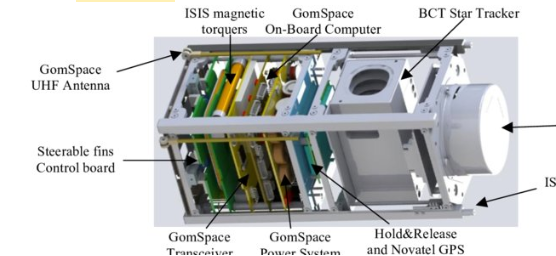
\includegraphics[scale=0.75]{Figures/Mechanical/example.png}
        \caption{BCT Star Tracker}
        \label{fig:sys_CAD}
    \end{figure}
    \item Modelling for the simulation of the extruded base to be changed from fixed support on bottom panel to fixed base plate and joints defined.
    \item Shell modelling to be incorporated in all simulations. Have to research on what is shell modelling and when it is used.
    \item Static loading to be changed to extreme case(as we do not know relative position with satellite) - (6g,6g,7g)-(7g,7g,7g) or otherwise doing all different simulations



\end{enumerate}

%----------------------------END----------------------------%
\end{document}
